\documentclass[aspectratio=169,11pt]{beamer}

% Compile with XeLaTeX
\usepackage{fontspec}
\setsansfont{DejaVu Sans}
\setmonofont{DejaVu Sans Mono}
\usepackage{polyglossia}
\setdefaultlanguage{vietnamese}
\usepackage{booktabs}
\usepackage{array}
\usepackage{tabularx}
\usepackage{listings}
\usepackage{xcolor}
\usepackage{ragged2e}

% Graphics
\usepackage{graphicx}
\graphicspath{{images/}}

\usetheme{Madrid}
\usecolortheme{seahorse}
\setbeamertemplate{navigation symbols}{}
\setbeamertemplate{footline}[frame number]
\setbeamertemplate{itemize items}[circle]
\setbeamertemplate{enumerate items}[default]

\definecolor{codebg}{RGB}{248,248,248}
\definecolor{codekw}{RGB}{0,72,160}
\definecolor{codestr}{RGB}{150,60,30}
\definecolor{accent}{RGB}{0,90,150}

\lstset{
  basicstyle=\ttfamily\scriptsize,
  keywordstyle=\color{codekw}\bfseries,
  stringstyle=\color{codestr},
  backgroundcolor=\color{codebg},
  frame=single,
  breaklines=true,
  columns=fullflexible,
  showstringspaces=false,
  keepspaces=true,
  language=SQL
}

\newcommand{\keyword}[1]{\textcolor{accent}{\textbf{#1}}}
\newcommand{\tightlist}{\setlength{\itemsep}{2pt}\setlength{\parskip}{0pt}}
\newcommand{\qoption}[2]{\item[#1.] #2}

\title[Introduction to Databases]{Introduction to Databases}
\subtitle{Database, DBMS, RDBMS, NoSQL, and ACID}
\author{Lecture Notes}
\institute{Course: Databases}
\date{Updated: 28/04/2026}

\begin{document}

%------------------------------------------------
\begin{frame}
  \titlepage
\end{frame}

%------------------------------------------------
\begin{frame}{Learning Objectives}
\small
After this lesson, learners will be able to:
\begin{enumerate}
\tightlist
  \item Explain the concepts of \keyword{data} and \keyword{database}.
  \item Describe the role of a \keyword{DBMS} in storing, retrieving, and managing data.
  \item Describe the main components of a database.
  \item Distinguish between \keyword{Relational Databases} and \keyword{NoSQL Databases}.
  \item Explain the meaning of the \keyword{ACID} properties.
  \item Identify real-world applications of databases in different domains.
  \item Select suitable database types for selected technology domains.
\end{enumerate}
\end{frame}

%------------------------------------------------
\begin{frame}{Data and Information}
\small
\begin{block}{Data}
Data consists of raw facts, figures, or information that has not yet been organized and has little meaning when considered alone.
\end{block}

\begin{columns}[T]
\column{0.48\textwidth}
Examples of data:
\begin{itemize}
\tightlist
  \item Customer name
  \item Phone number
  \item Student ID
  \item Exam score
  \item Transaction date
  \item Images, videos, and audio
\end{itemize}

\column{0.48\textwidth}
\begin{block}{Information}
When data is processed, organized, and analyzed, it becomes meaningful information that supports decision-making.
\end{block}
\end{columns}
\end{frame}

%------------------------------------------------
\begin{frame}{What is a database?}
\small
\begin{block}{Definition}
A database is a structured system used to \textbf{store}, \textbf{manage}, \textbf{retrieve}, and \textbf{update} data efficiently for multiple users and applications.
\end{block}

Databases are important because:
\begin{itemize}
\tightlist
  \item \keyword{Scalability}: handles large volumes of data.
  \item \keyword{Data Integrity}: maintains accuracy through rules and constraints.
  \item \keyword{Security}: protects data through access rights and permissions.
  \item \keyword{Analytics}: supports analysis and decision-making.
\end{itemize}
\end{frame}

\begin{frame}{Illustration: Why Databases Matter}
\centering
\vfill
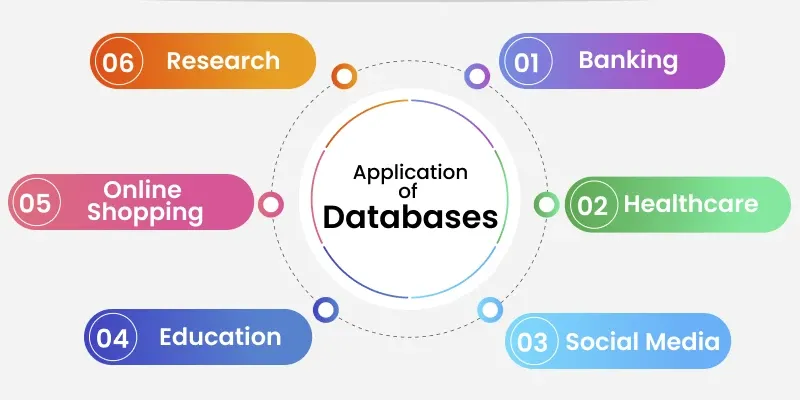
\includegraphics[width=0.78\textwidth,height=0.68\textheight,keepaspectratio]{image-4.png}
\vfill
\end{frame}

%------------------------------------------------
\begin{frame}{Quiz: Data and Database Concepts}
\small
\textbf{Question 1.} What is data?
\begin{enumerate}
\tightlist
  \qoption{A}{Fully analyzed information}
  \qoption{B}{Raw facts, figures, or unprocessed information}
  \qoption{C}{A data management software package}
  \qoption{D}{A type of programming language}
\end{enumerate}

\textbf{Question 2.} What is a database mainly used for?
\begin{enumerate}
\tightlist
  \qoption{A}{Designing user interfaces}
  \qoption{B}{Storing, managing, and retrieving data}
  \qoption{C}{Only for writing Python programs}
  \qoption{D}{Only for storing images}
\end{enumerate}
\end{frame}

%------------------------------------------------
\begin{frame}{Quiz: Data and Database Concepts (cont.)}
\small
\textbf{Question 3.} Which feature helps a database handle large volumes of data?
\begin{enumerate}
\tightlist
  \qoption{A}{Security}
  \qoption{B}{Scalability}
  \qoption{C}{Isolation}
  \qoption{D}{Durability}
\end{enumerate}
\end{frame}

%------------------------------------------------
\begin{frame}{How Databases Work}
\small
Databases organize and store information in structured or unstructured formats, allowing users to easily:
\begin{itemize}
\tightlist
  \item Access, search for, and retrieve data.
  \item Update, delete, and manage data.
  \item Manage access permissions.
\end{itemize}

\begin{block}{The Central Role of a DBMS}
A DBMS is a software layer between users and raw data. Users interact with the DBMS through queries or applications instead of directly handling physical storage details.
\end{block}
\end{frame}

%------------------------------------------------
\begin{frame}{Request Processing in a DBMS}
\small
\begin{enumerate}
\tightlist
  \item A user or application sends a request to the DBMS.
  \item The DBMS checks syntax, verifies access rights, and optimizes the query.
  \item The DBMS accesses relevant data from tables, indexes, or storage files.
  \item The DBMS returns results to the user or application.
\end{enumerate}

\vspace{0.2cm}
The DBMS also provides:
\begin{itemize}
\tightlist
  \item Data backup and recovery.
  \item Performance optimization.
  \item Transaction management.
  \item Access control.
  \item Concurrent multi-user management.
\end{itemize}
\end{frame}

\begin{frame}{Illustration: Request Processing in a DBMS}
\centering
\vfill
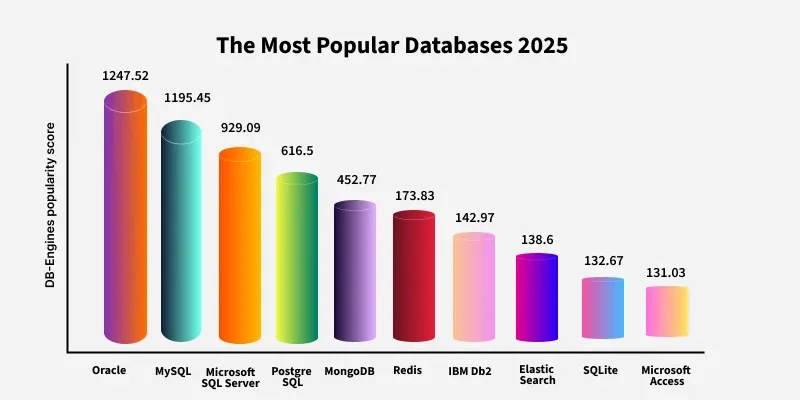
\includegraphics[width=0.80\textwidth,height=0.66\textheight,keepaspectratio]{image-5.png}
\vfill
\end{frame}

%------------------------------------------------
\begin{frame}{Quiz: How Databases Work}
\small
\textbf{Question 1.} What role does a DBMS play in a database system?
\begin{enumerate}
\tightlist
  \qoption{A}{It is an intermediary layer between users and data}
  \qoption{B}{It is a hardware device used to store data}
  \qoption{C}{It is a programming language that replaces SQL}
  \qoption{D}{It is software used only for drawing charts}
\end{enumerate}

\textbf{Question 2.} When a user submits a query, what does the DBMS usually do?
\begin{enumerate}
\tightlist
  \qoption{A}{Ignores the query}
  \qoption{B}{Processes the query, finds relevant data, and returns results}
  \qoption{C}{Always deletes data before returning results}
  \qoption{D}{Only saves the query into a text file}
\end{enumerate}
\end{frame}

%------------------------------------------------
\begin{frame}{Quiz: How Databases Work (cont.)}
\small
\textbf{Question 3.} Which of the following is an important DBMS function?
\begin{enumerate}
\tightlist
  \qoption{A}{Data backup and recovery}
  \qoption{B}{Only playing music}
  \qoption{C}{Only image editing}
  \qoption{D}{Only compiling C++ programs}
\end{enumerate}
\end{frame}

%------------------------------------------------

\begin{frame}{Components of a Database}
\small
A database consists of multiple components that work together to store, organize, manage, and retrieve data efficiently.

\vspace{0.25cm}
\begin{tabularx}{\textwidth}{>{\bfseries}p{0.24\textwidth} X}
\toprule
Component & Main role \\
\midrule
Data & The actual information stored in the database. \\
Schema & The blueprint that describes how data is organized. \\
DBMS & Software that manages database operations. \\
Query & Instructions used to retrieve, add, update, or delete data. \\
Users & Individuals or systems that interact with the database. \\
\bottomrule
\end{tabularx}
\end{frame}

\begin{frame}{Illustration: Database Components}
\centering
\vfill
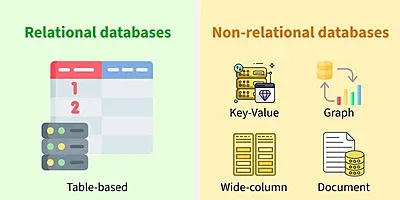
\includegraphics[width=0.84\textwidth,height=0.62\textheight,keepaspectratio]{image-6.png}
\vfill
\end{frame}

%------------------------------------------------
\begin{frame}{Component 1: Data}
\small
\begin{block}{Concept}
\keyword{Data} is the actual information stored in the database.
\end{block}

Data may include:
\begin{itemize}
\tightlist
  \item Text, numbers, and dates.
  \item Images, files, audio, and video.
  \item Sensor data or system-generated data.
\end{itemize}

\begin{exampleblock}{Example}
In a student management system, data may include student ID, full name, date of birth, class, exam scores, and academic status.
\end{exampleblock}
\end{frame}

%------------------------------------------------
\begin{frame}{Component 2: Database Schema}
\small
\begin{block}{Schema}
A \keyword{schema}, or \keyword{database schema}, is the blueprint that describes how data is organized.
\end{block}

A schema may describe:
\begin{itemize}
\tightlist
  \item Tables and fields.
  \item The data type of each field.
  \item Primary keys and foreign keys.
  \item Relationships between tables.
  \item Data constraints.
\end{itemize}
\end{frame}

%------------------------------------------------
\begin{frame}{Example of a Database Schema}
\small
In a sales management database, the schema may include the following tables:

\begin{itemize}
\tightlist
  \item \texttt{Customers}: stores customer information.
  \item \texttt{Orders}: stores order information.
  \item \texttt{Products}: stores product information.
  \item \texttt{OrderDetails}: stores line-item details for each order.
\end{itemize}

\begin{block}{Meaning}
A schema tells the system how data is organized, how tables are connected, and which constraints the data must satisfy.
\end{block}
\end{frame}

%------------------------------------------------
\begin{frame}{Component 3: Database Management System}
\small
\begin{block}{DBMS}
A \keyword{DBMS} is software that manages database operations.
\end{block}

A DBMS supports functions such as:
\begin{itemize}
\tightlist
  \item Storing, retrieving, updating, and deleting data.
  \item Managing security and users.
  \item Transaction management.
  \item Data backup and recovery.
\end{itemize}
\end{frame}

%------------------------------------------------
\begin{frame}{Examples of DBMSs}
\small
Some popular database management systems:

\begin{columns}[T]
\column{0.5\textwidth}
\begin{itemize}
\tightlist
  \item MySQL.
  \item PostgreSQL.
  \item Oracle.
\end{itemize}

\column{0.5\textwidth}
\begin{itemize}
\tightlist
  \item Microsoft SQL Server.
  \item MongoDB.
\end{itemize}
\end{columns}

\vspace{0.25cm}
\begin{block}{Remember}
A DBMS does not only store data; it also controls how data is accessed, protected, updated, and recovered after failures.
\end{block}
\end{frame}

\begin{frame}{Illustration: Database Management System}
\centering
\vfill
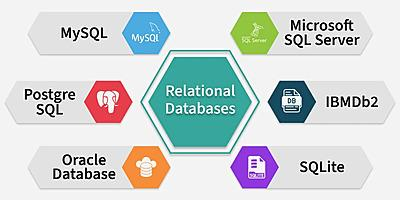
\includegraphics[width=0.84\textwidth,height=0.62\textheight,keepaspectratio]{image-7.png}
\vfill
\end{frame}

%------------------------------------------------
\begin{frame}[fragile]{Component 4: Query}
\small
\begin{block}{Query}
A \keyword{query} is an instruction used to retrieve, add, update, or delete data in a database.
\end{block}

In relational databases, queries are usually written in \keyword{SQL}.

\begin{lstlisting}
SELECT * FROM Students
WHERE major = 'Data Science';
\end{lstlisting}

The query above retrieves the list of students majoring in \textit{Data Science}.
\end{frame}

%------------------------------------------------
\begin{frame}{Component 5: Users}
\small
Users are individuals or systems that interact with a database.

\vspace{0.15cm}
Common user groups include:
\begin{itemize}
\tightlist
  \item Database administrators.
  \item Developers.
  \item Data analysts.
  \item End users.
  \item Software applications.
  \item Automated systems.
\end{itemize}

\begin{block}{Authorization}
Each user group may have different access privileges depending on its role.
\end{block}
\end{frame}

%------------------------------------------------
\begin{frame}{Two Common Database Groups}
\small
\begin{columns}[T]
\column{0.48\textwidth}
\begin{block}{Relational Database}
\begin{itemize}
\tightlist
  \item Organizes data into tables.
  \item Has rows, columns, primary keys, and foreign keys.
  \item Commonly uses SQL.
  \item Suitable for structured data.
\end{itemize}
\end{block}

\column{0.48\textwidth}
\begin{block}{NoSQL Database}
\begin{itemize}
\tightlist
  \item More flexible in data models.
  \item Suitable for unstructured or semi-structured data.
  \item Supports horizontal scalability well.
  \item Includes document, key-value, wide-column, and graph databases.
\end{itemize}
\end{block}
\end{columns}
\end{frame}

%------------------------------------------------
\begin{frame}{Relational Databases}
\small
A \keyword{Relational Database} organizes data into tables. Each table includes:
\begin{itemize}
\tightlist
  \item \textbf{Rows/Records}: specific records.
  \item \textbf{Columns/Fields}: attributes of the records.
\end{itemize}

\begin{table}[]
\centering
\scriptsize
\begin{tabular}{llll}
\toprule
StudentID & FullName & Major & GPA \\
\midrule
S001 & Nguyen An & Data Science & 3.4 \\
S002 & Tran Binh & AI & 3.7 \\
S003 & Le Chi & Information Systems & 3.2 \\
\bottomrule
\end{tabular}
\end{table}
\end{frame}

%------------------------------------------------
\begin{frame}{Characteristics of Relational Databases}
\small
\begin{itemize}
\tightlist
  \item \textbf{Strict schema}: tables, columns, data types, and constraints are predefined.
  \item \textbf{Primary key}: uniquely identifies each record in a table.
  \item \textbf{Foreign key}: represents relationships between tables.
  \item \textbf{ACID}: ensures reliable transactions.
  \item \textbf{Structured data}: suitable for accounting, banking, student management, and sales.
\end{itemize}

Examples of RDBMSs: MySQL, PostgreSQL, Oracle, and Microsoft SQL Server.
\end{frame}

%------------------------------------------------
\begin{frame}{Quiz: Relational Databases}
\small
\textbf{Question 1.} How do relational databases mainly organize data?
\begin{enumerate}
\tightlist
  \qoption{A}{Graphs}
  \qoption{B}{Tables with rows and columns}
  \qoption{C}{Audio files}
  \qoption{D}{Blockchain}
\end{enumerate}

\textbf{Question 2.} What is a primary key used for?
\begin{enumerate}
\tightlist
  \qoption{A}{Uniquely identifying each record in a table}
  \qoption{B}{Deleting the entire database}
  \qoption{C}{Encrypting images}
  \qoption{D}{Creating a user interface}
\end{enumerate}
\end{frame}

%------------------------------------------------
\begin{frame}{Quiz: Relational Databases (cont.)}
\small
\textbf{Question 3.} Which of the following is an RDBMS?
\begin{enumerate}
\tightlist
  \qoption{A}{PostgreSQL}
  \qoption{B}{Redis}
  \qoption{C}{Neo4j}
  \qoption{D}{IPFS}
\end{enumerate}
\end{frame}

%------------------------------------------------
\begin{frame}{NoSQL Databases}
\small
\keyword{NoSQL} stands for \textit{Not Only SQL}. NoSQL databases are designed to handle unstructured or semi-structured data such as:
\begin{itemize}
\tightlist
  \item Text, images, and videos.
  \item Sensor data.
  \item Log system.
  \item Social media data.
  \item Real-time data.
\end{itemize}

Unlike RDBMSs, NoSQL databases do not necessarily store data in fixed tables.
\end{frame}

%------------------------------------------------
\begin{frame}{Main Types of NoSQL Databases}
\small
\begin{tabularx}{\textwidth}{>{\bfseries}p{0.24\textwidth} X p{0.22\textwidth}}
\toprule
Type & Description & Example \\
\midrule
Document & Stores data as JSON-like documents & MongoDB \\
Key-value & Stores key-value pairs for fast lookup & Redis \\
Wide-column & Stores data by columns; suitable for big data & Cassandra \\
Graph & Stores nodes and relationships between nodes & Neo4j \\
\bottomrule
\end{tabularx}
\end{frame}

%------------------------------------------------
\begin{frame}{Quiz: NoSQL Databases}
\small
\textbf{Question 1.} What does NoSQL stand for?
\begin{enumerate}
\tightlist
  \qoption{A}{No Software Query Language}
  \qoption{B}{Not Only SQL}
  \qoption{C}{New Online SQL}
  \qoption{D}{Normal SQL}
\end{enumerate}

\textbf{Question 2.} Which NoSQL type stores data as key-value pairs?
\begin{enumerate}
\tightlist
  \qoption{A}{Document database}
  \qoption{B}{Key-value store}
  \qoption{C}{Graph database}
  \qoption{D}{Relational database}
\end{enumerate}
\end{frame}

%------------------------------------------------
\begin{frame}{Quiz: NoSQL Databases (cont.)}
\small
\textbf{Question 3.} Neo4j is an example of which type of database?
\begin{enumerate}
\tightlist
  \qoption{A}{Graph database}
  \qoption{B}{Key-value store}
  \qoption{C}{RDBMS}
  \qoption{D}{File system}
\end{enumerate}
\end{frame}

%------------------------------------------------
\begin{frame}{What Is ACID?}
\small
\keyword{ACID} consists of four important properties that make database transactions reliable, accurate, and safe.

\begin{tabularx}{\textwidth}{>{\bfseries}p{0.22\textwidth} X}
\toprule
Property & Meaning \\
\midrule
Atomicity & A transaction must be executed completely or not at all. \\
Consistency & The database moves from one valid state to another valid state. \\
Isolation & Concurrent transactions do not incorrectly affect one another. \\
Durability & After a transaction is completed, changes are stored permanently. \\
\bottomrule
\end{tabularx}
\end{frame}

%------------------------------------------------
\begin{frame}{ACID Example: Bank Transfer}
\small
When transferring money from account A to account B:
\begin{enumerate}
\tightlist
  \item Debit account A.
  \item Credit account B.
\end{enumerate}

\begin{itemize}
\tightlist
  \item \textbf{Atomicity}: if step 2 fails, step 1 must be rolled back.
  \item \textbf{Consistency}: the balance remains valid after the transaction.
  \item \textbf{Isolation}: concurrent transactions do not corrupt the data.
  \item \textbf{Durability}: a successful transaction must be stored permanently.
\end{itemize}
\end{frame}

%------------------------------------------------
\begin{frame}{Quiz: ACID Properties}
\small
\textbf{Question 1.} Which properties does ACID include?
\begin{enumerate}
\tightlist
  \qoption{A}{Accuracy, Control, Integrity, Design}
  \qoption{B}{Atomicity, Consistency, Isolation, Durability}
  \qoption{C}{Access, Cache, Index, Data}
  \qoption{D}{Application, Cloud, Internet, Database}
\end{enumerate}

\textbf{Question 2.} Which property ensures that a transaction is executed completely or not at all?
\begin{enumerate}
\tightlist
  \qoption{A}{Atomicity}
  \qoption{B}{Consistency}
  \qoption{C}{Isolation}
  \qoption{D}{Durability}
\end{enumerate}
\end{frame}

%------------------------------------------------
\begin{frame}{Quiz: ACID Properties (cont.)}
\small
\textbf{Question 3.} Which property ensures that data remains stored after a transaction has completed?
\begin{enumerate}
\tightlist
  \qoption{A}{Atomicity}
  \qoption{B}{Consistency}
  \qoption{C}{Isolation}
  \qoption{D}{Durability}
\end{enumerate}
\end{frame}

%------------------------------------------------
\begin{frame}{Real-World Applications of Databases}
\small
\begin{tabularx}{\textwidth}{>{\bfseries}p{0.23\textwidth} X}
\toprule
Domain & Commonly managed data \\
\midrule
Banking & Transactions, accounts, loans, and customer information. \\
Transportation & Bookings, schedules, routes, vehicles, and passengers. \\
Education & Student records, grades, schedules, and tuition fees. \\
Retail & Inventory, orders, customers, promotions, and revenue. \\
Social media & Users, posts, messages, images, videos, and interactions. \\
\bottomrule
\end{tabularx}
\end{frame}

%------------------------------------------------
\begin{frame}{Quiz: Database Applications}
\small
\textbf{Question 1.} In banking, what are databases commonly used to store?
\begin{enumerate}
\tightlist
  \qoption{A}{Transactions and accounts}
  \qoption{B}{Only desktop wallpapers}
  \qoption{C}{Only program source code}
  \qoption{D}{Only audio files}
\end{enumerate}

\textbf{Question 2.} In education, what can databases be used to manage?
\begin{enumerate}
\tightlist
  \qoption{A}{Student records and grades}
  \qoption{B}{Computer fan speed}
  \qoption{C}{TV control signals}
  \qoption{D}{Interface colors}
\end{enumerate}
\end{frame}

%------------------------------------------------
\begin{frame}{Quiz: Database Applications (cont.)}
\small
\textbf{Question 3.} In retail, what can databases help manage?
\begin{enumerate}
\tightlist
  \qoption{A}{Inventory and orders}
  \qoption{B}{Only personal videos}
  \qoption{C}{Only router IP addresses}
  \qoption{D}{Only music players}
\end{enumerate}
\end{frame}

%------------------------------------------------
\begin{frame}{Databases in Technology Domains}
\small
\begin{itemize}
\tightlist
  \item \textbf{Web Development}: MySQL, PostgreSQL, MongoDB, Firebase.
  \item \textbf{Mobile Development}: SQLite, Realm, Firebase Realtime Database.
  \item \textbf{DevOps}: PostgreSQL, Redis, InfluxDB, Cassandra.
  \item \textbf{Data Engineering}: HDFS, Cassandra, Redshift, BigQuery.
  \item \textbf{Data Science}: PostgreSQL, MongoDB, Hive, Snowflake.
  \item \textbf{AI}: MongoDB, Cassandra, BigQuery, AWS S3.
  \item \textbf{Cloud}: Aurora, Cloud Spanner, Azure Cosmos DB.
  \item \textbf{Blockchain/Web3}: BigchainDB, IPFS, Ethereum, Chainlink.
\end{itemize}
\end{frame}

%------------------------------------------------
\begin{frame}{Quiz: Databases by Technology Domain}
\small
\textbf{Question 1.} Which database is often used in mobile applications because it is lightweight and suitable for local storage?
\begin{enumerate}
\tightlist
  \qoption{A}{SQLite}
  \qoption{B}{Oracle RAC}
  \qoption{C}{HDFS}
  \qoption{D}{Ethereum}
\end{enumerate}

\textbf{Question 2.} Which domain is Google BigQuery commonly suitable for?
\begin{enumerate}
\tightlist
  \qoption{A}{Data engineering and big data analytics}
  \qoption{B}{Only image editing}
  \qoption{C}{Small offline game programming}
  \qoption{D}{Keyboard control}
\end{enumerate}
\end{frame}

%------------------------------------------------
\begin{frame}{Quiz: Databases by Technology Domain (cont.)}
\small
\textbf{Question 3.} Which field is IPFS commonly associated with?
\begin{enumerate}
\tightlist
  \qoption{A}{Blockchain/Web3}
  \qoption{B}{Traditional classroom management}
  \qoption{C}{Only personal desktop applications}
  \qoption{D}{The Windows operating system}
\end{enumerate}
\end{frame}

%------------------------------------------------
\begin{frame}{Comparison: Relational Database vs. NoSQL}
\scriptsize
\begin{tabularx}{\textwidth}{>{\bfseries}p{0.20\textwidth} X X}
\toprule
Criterion & Relational Database & NoSQL Database \\
\midrule
Structure & Tables, rows, columns & Documents, key-value, wide-column, graphs \\
Schema & Usually fixed and strict & More flexible \\
Language & SQL & Depends on the DBMS \\
Relationships & Primary keys, foreign keys, joins & Depends on the data model \\
Scalability & Usually strong in vertical scaling & Usually strong in horizontal scaling \\
Suitable for & Structured data & Unstructured/semi-structured data \\
Examples & MySQL, PostgreSQL, Oracle & MongoDB, Redis, Cassandra, Neo4j \\
\bottomrule
\end{tabularx}
\end{frame}

%------------------------------------------------
\begin{frame}{Review Questions: Multiple Choice}
\small
\textbf{Question 1.} What is a database?
\begin{enumerate}
\tightlist
  \qoption{A}{A system used to store, manage, and retrieve data}
  \qoption{B}{A web browser}
  \qoption{C}{An operating system}
  \qoption{D}{An input device}
\end{enumerate}

\textbf{Question 2.} What is a DBMS?
\begin{enumerate}
\tightlist
  \qoption{A}{Software for managing databases}
  \qoption{B}{A type of monitor}
  \qoption{C}{A social network protocol}
  \qoption{D}{Software used only for drawing images}
\end{enumerate}
\end{frame}

%------------------------------------------------
\begin{frame}{Review Questions: Multiple Choice (cont.)}
\small
\textbf{Question 3.} Which component describes table, field, and relationship structures?
\begin{enumerate}
\tightlist
  \qoption{A}{Schema}
  \qoption{B}{User}
  \qoption{C}{Query}
  \qoption{D}{Image file}
\end{enumerate}

\textbf{Question 4.} What do relational databases organize data into?
\begin{enumerate}
\tightlist
  \qoption{A}{Tables}
  \qoption{B}{Video}
  \qoption{C}{Voice messages}
  \qoption{D}{An unstructured random bit string}
\end{enumerate}
\end{frame}

%------------------------------------------------
\begin{frame}{Review Questions: Multiple Choice (cont.)}
\small
\textbf{Question 5.} What type of data is NoSQL suitable for?
\begin{enumerate}
\tightlist
  \qoption{A}{Unstructured or semi-structured data}
  \qoption{B}{Only rigid tabular data}
  \qoption{C}{Only small integers}
  \qoption{D}{Only data printed on paper}
\end{enumerate}

\textbf{Question 6.} What does the Isolation property in ACID mean?
\begin{enumerate}
\tightlist
  \qoption{A}{Concurrent transactions do not interfere with each other incorrectly}
  \qoption{B}{Data is never stored}
  \qoption{C}{Every table must have an illustration}
  \qoption{D}{Queries must be written in Vietnamese}
\end{enumerate}
\end{frame}

%------------------------------------------------
\begin{frame}{Review Questions: Multiple Choice (cont.)}
\small
\textbf{Question 7.} MongoDB is an example of which database type?
\begin{enumerate}
\tightlist
  \qoption{A}{Document database}
  \qoption{B}{Graph database}
  \qoption{C}{Key-value store}
  \qoption{D}{Traditional relational database}
\end{enumerate}

\textbf{Question 8.} What is Redis commonly used for?
\begin{enumerate}
\tightlist
  \qoption{A}{Caching or fast key-value lookup}
  \qoption{B}{Designing presentation slides}
  \qoption{C}{Drawing 3D models}
  \qoption{D}{Only storing long videos}
\end{enumerate}
\end{frame}

%------------------------------------------------
\begin{frame}{Review Questions: Multiple Choice (cont.)}
\small
\textbf{Question 9.} What kind of problems is Neo4j suitable for?
\begin{enumerate}
\tightlist
  \qoption{A}{Relationship and graph analysis}
  \qoption{B}{Calculating payroll on paper}
  \qoption{C}{Storing simple local music files}
  \qoption{D}{Only editing text}
\end{enumerate}

\textbf{Question 10.} In AI, what can databases be used for?
\begin{enumerate}
\tightlist
  \qoption{A}{Storing training datasets and model feedback}
  \qoption{B}{Only setting application background colors}
  \qoption{C}{Completely replacing machine learning algorithms}
  \qoption{D}{Only managing the mouse and keyboard}
\end{enumerate}
\end{frame}

%------------------------------------------------
\begin{frame}{Review Questions: Short Answer}
\small
\begin{enumerate}
\tightlist
  \item Distinguish between data and information.
  \item Explain the role of a DBMS in a database system.
  \item Why are relational databases suitable for structured data?
  \item Why is NoSQL suitable for big data, unstructured data, or rapidly changing data?
  \item Explain the meaning of the four ACID properties using a real-world example.
\end{enumerate}
\end{frame}

%------------------------------------------------
\begin{frame}{Practice Exercises}
\small
\begin{block}{Exercise 1}
A university wants to build a student management system including student information, classes, courses, grades, and tuition fees. Propose a suitable database type and explain your choice.
\end{block}

\begin{block}{Exercise 2}
A social network needs to store user profiles, posts, comments, images, videos, and friendship relationships. Propose one or more suitable database types.
\end{block}
\end{frame}

%------------------------------------------------
\begin{frame}{Further Practice Exercises}
\small
\begin{block}{Exercise 3}
An e-commerce application needs to store products, orders, customers, payments, and purchase history. Should it combine a relational database and NoSQL? Why?
\end{block}

\begin{block}{Exercise 4}
An AI system needs to store training datasets consisting of text, images, and real-time user feedback. Propose a suitable data storage architecture.
\end{block}
\end{frame}

%------------------------------------------------
\begin{frame}{Lesson Summary}
\small
\begin{itemize}
\tightlist
  \item Data is raw information; databases help organize and manage data efficiently.
  \item A DBMS is intermediary software that helps users and applications interact with data.
  \item A database consists of data, schema, DBMS, queries, and users.
  \item RDBMSs organize data in tables and are suitable for structured data.
  \item NoSQL is suitable for unstructured data, semi-structured data, and systems requiring horizontal scaling.
  \item ACID helps ensure that database transactions are reliable, accurate, and safe.
\end{itemize}
\end{frame}

%------------------------------------------------
\begin{frame}{Key Terms}
\small
\begin{columns}[T]
\column{0.48\textwidth}
\begin{itemize}
\tightlist
  \item Data, Information, Database
  \item DBMS, Schema, Query, SQL
  \item Relational Database, RDBMS
  \item NoSQL, Document Database
  \item Key-Value Store
  \item Wide-Column Database
\end{itemize}
\column{0.48\textwidth}
\begin{itemize}
\tightlist
  \item Graph Database
  \item ACID
  \item Atomicity, Consistency
  \item Isolation, Durability
  \item Data Engineering, Data Science
  \item AI, Cloud, Blockchain, Web3
\end{itemize}
\end{columns}
\end{frame}

%------------------------------------------------
\begin{frame}
\centering
\Huge Thank you!\\[0.5cm]
\Large Discussion and Questions
\end{frame}

\end{document}

